\documentclass[a4paper,12pt,titlepage]{article}

\usepackage{amsmath,amsthm,amssymb}
\usepackage{enumerate}
\usepackage{hyperref}
\usepackage{graphicx}


\oddsidemargin -0.65cm
\evensidemargin -0.65cm

\textwidth 17cm
\textheight 26cm

\begin{document}

\setlength{\tabcolsep}{0.015\textwidth}
\begin{center} \begin{tabular}{cccc}
	
\includegraphics[width=0.16\textwidth]{SAMF_logo.jpg} &
	
\includegraphics[width=0.35\textwidth]{SAICA_logo.jpg} &
	
\includegraphics[width=0.18\textwidth]{Liberty_logo.jpg} &
	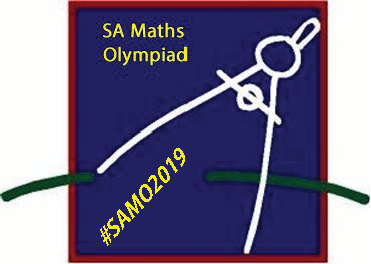
\includegraphics[width=0.18\textwidth]{SAMO2019.png}
\end{tabular} \end{center}


\vspace{30pt}

\begin{center}
\textbf{\Large Intermediate February Monthly Problem Set}
\\ \vspace{1em}
\textbf{\large Due: 28 February 2019}
\end{center}

\vspace{4pt}

\begin{enumerate}[1.]

\item %Estonia 2000/2001 National Round Grade 9 Q1
Sophie had to solve a math problem in the class. While cleaning the blackboard, she accidentally erased a part of her problem as well: the text that remained on board was $37\cdot(72+3x)=14{**}45$, where $*$ marks an erased digit. Show that Sophie can still solve her problem, knowing that $x$ is an integer.


\item %Romania 2017 District Round Grade 7 Q3
On the side $CD$ of square $ABCD$ point $E$ is chosen such that $\angle ABE = 60^{\circ}$. Point $F$ is chosen on line $AB$ such that $BE = BF$ and point $A$ is between $F$ and $B$. Let $M$ be the intersection of lines $EF$ and $AD$.
\begin{itemize}
\item [a)] Find $\angle BME$.
\item [b)] The bisector of angle $CBE$ intersects $CD$ at $N$. Find the angles of triangle $BMN$.
\end{itemize}


\item % Estonia National Olympiad 2005/2006 Grade 9
Let there be $n \geq 2$ real numbers such that none of them is greater than the arithmetic mean (normal average) of the other numbers. Prove that all the numbers are equal.


\item %Romania 2017 Final Round Grade 6 Q2
Consider the isosceles triangle $ABC$ with $\angle A = 100^{\circ}$. Let $BD$ be the angle bisector of $\angle ABC$ with $D$ a point on $AC$. Let $E$ be a point on $BD$ such that $BE=BC$ and where $D$ is between points $B$ and $E$. Let $F$ be a point on $BC$ with $F$ between $B$ and $C$ such that $AB=BF$. Prove that the lines $AC$ and $EF$ are perpendicular.


\item %Russia 2014 Grade 9 Q3
The teacher gave Emma four distinct integers and asked Emma to calculate the greatest common divisor of every two of these numbers. She got the answers 1, 2, 3, 4, 5 and $N$ where $N>5$. What is the smallest possible value of $N$?


\item %Estonia 2000/2001 National Round Grade 9 Q5
A table consisting of $9$ rows and $2001$ columns is filled with integers $1,\,2,\,\ldots,\,2001$ in such a way that each of these integers occurs in the table exactly $9$ times and the integers in any column differ by no more than $3$. Find the maximum possible value of the minimal column sum (sum of the numbers in one column).


%\item % IPMO 2006 Junior Individual Q5
%If $a = 2^{2006} + 2^{-2006}$ and $b = 2^{2006} - 2^{-2006}$ then what is the value of $a^2 - b^2$?


%\item % IPMO 2008 Junior Individual Q11
%Paul likes dogs. At present all his adult dogs are Dalmatians while some of his puppies are Dalmatians and some are not. In all he has 11 dogs of which 7 are Dalmatians and 8 are puppies. How many Dalmatian puppies has he?


%\item % IPMO 2006 Junior Team Q6
%How many distinct factors does 1 000 000 000 have?


%\item % IPMO 2008 Junior Team Q9
%If a regular octagon has side length 1 cm, find the distance between the opposite sides.


\item % SW-2013-3
Let $n$ be a positive integer. Both $n$ and $n^2$ only contain the digits $1$, $2$ and $3$ (not necessarily all of them). Determine all possible values of $n$.


%\item % DB-2012-2
%Given a (not necessarily convex) quadrilateral $ABCD$, call a point $P$ in the same plane as $ABCD$ an \emph{areal centre} for $ABCD$, if any line through $P$ divides $ABCD$ into two parts of equal area. What are necessary and sufficient conditions on $ABCD$ for it to possess an areal centre?


\item % The Liam
The (English language version of the) game of Scrabble\texttrademark{} consists of 100 tiles, each containing either a letter from A to Z (some letters occur more than once), except for two blank tiles; see \href{https://en.wikipedia.org/wiki/Scrabble_letter_distributions#English}{\texttt{the relevant Wikipedia page}} for the exact distribution of multiplicities of each letter.

In a solo game of Scrabble, the player starts by choosing seven tiles from the 100 available tiles at random. What is the probability that the player picks up exactly two vowels?


\end{enumerate}

\newpage

\vfill
\textbf{\Large Email submission guidelines}
\begin{itemize}
	\item Email your solutions to \href{mailto:samf.training.assignments@gmail.com}{\texttt{samf.training.assignments@gmail.com}}.
	\item In the subject of your email, include your name and the level of the assignment (Beginner, Intermediate or Senior).
	\item Submit each question in a single separate PDF file (with multiple pages if necessary), with your name and the question number written on each page.
	\item If you take photographs of your work, use a document scanner such as CamScanner to convert to PDF.
	\item If you have multiple PDF files for a question, combine them using software such as PDFsam.
\end{itemize}

\end{document}
